
\textbf{P4)} Considere un sistema formado por un resorte ideal de constante elástica $k$ con su extremo superior fijo y, unido al extremo inferior del resorte, una masa puntual $m$. De la masa $m$ cuelga, mediante una cuerda inextensible y de masa despreciable de longitud $\ell$, una segunda masa puntual de igual valor $m$.

El sistema oscila verticalmente bajo la acción de la gravedad. Sea $x(t)$ el desplazamiento vertical del conjunto respecto a su posición de equilibrio (tomando hacia abajo como sentido positivo).

\begin{enumerate}[a)]
	\item Usando la segunda ley de Newton, escriba las ecuaciones de movimiento para cada masa y obtenga la ecuación efectiva para $x(t)$ (pequeñas oscilaciones alrededor del equilibrio).
	\item Determine la frecuencia angular $\omega$ de las pequeñas oscilaciones y escriba la solución general para $x(t)$, $v(t)$ y $a(t)$.
	\item Suponga que el sistema se suelta desde el reposo con una elongación inicial $x(0)=A$ (desde la posición de equilibrio). Determine la condición crítica sobre $A$ para la cual la cuerda puede llegar a perder tensión en algún instante del movimiento. Indique los pasos para encontrar la posición de equilibrio usada en los cálculos.
\end{enumerate}
\textbf{Hint:} Use h+x como la longitud del resorte, Determine primero la posición de equilibrio
\vspace{0.3cm}

\vspace{0.3cm}
\begin{center}
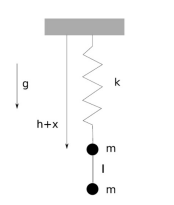
\includegraphics[width=0.32\textwidth]{imagenes/imagenp4a7.PNG}
\end{center}
